
The model we consider is the current draft specification \cite{ECMA} of the ECMAScript standard. 
This draft as far as the memory model goes has remained unchanged, so we believe our work will also be of use to those working on it. 
The specification is claimed to be axiomatic by definition, which should, in our view remove the complexities of the rest of the standard from the semantics of the model.
However, there were some concerns with it: 

\paragraph{The Model is Quite Algorithmic}
    Although the standard states that the model is not supposed to be operational, the specifications of the model hint otherwise. 
    There are quite a few abstract operations which are not necessary to understand the semantics of the model. 
    As an example, consider one of the Axioms of the model in Figure~\ref{model:Std1} as stated by the standard. 
    \begin{figure}[H]
        \centering 
        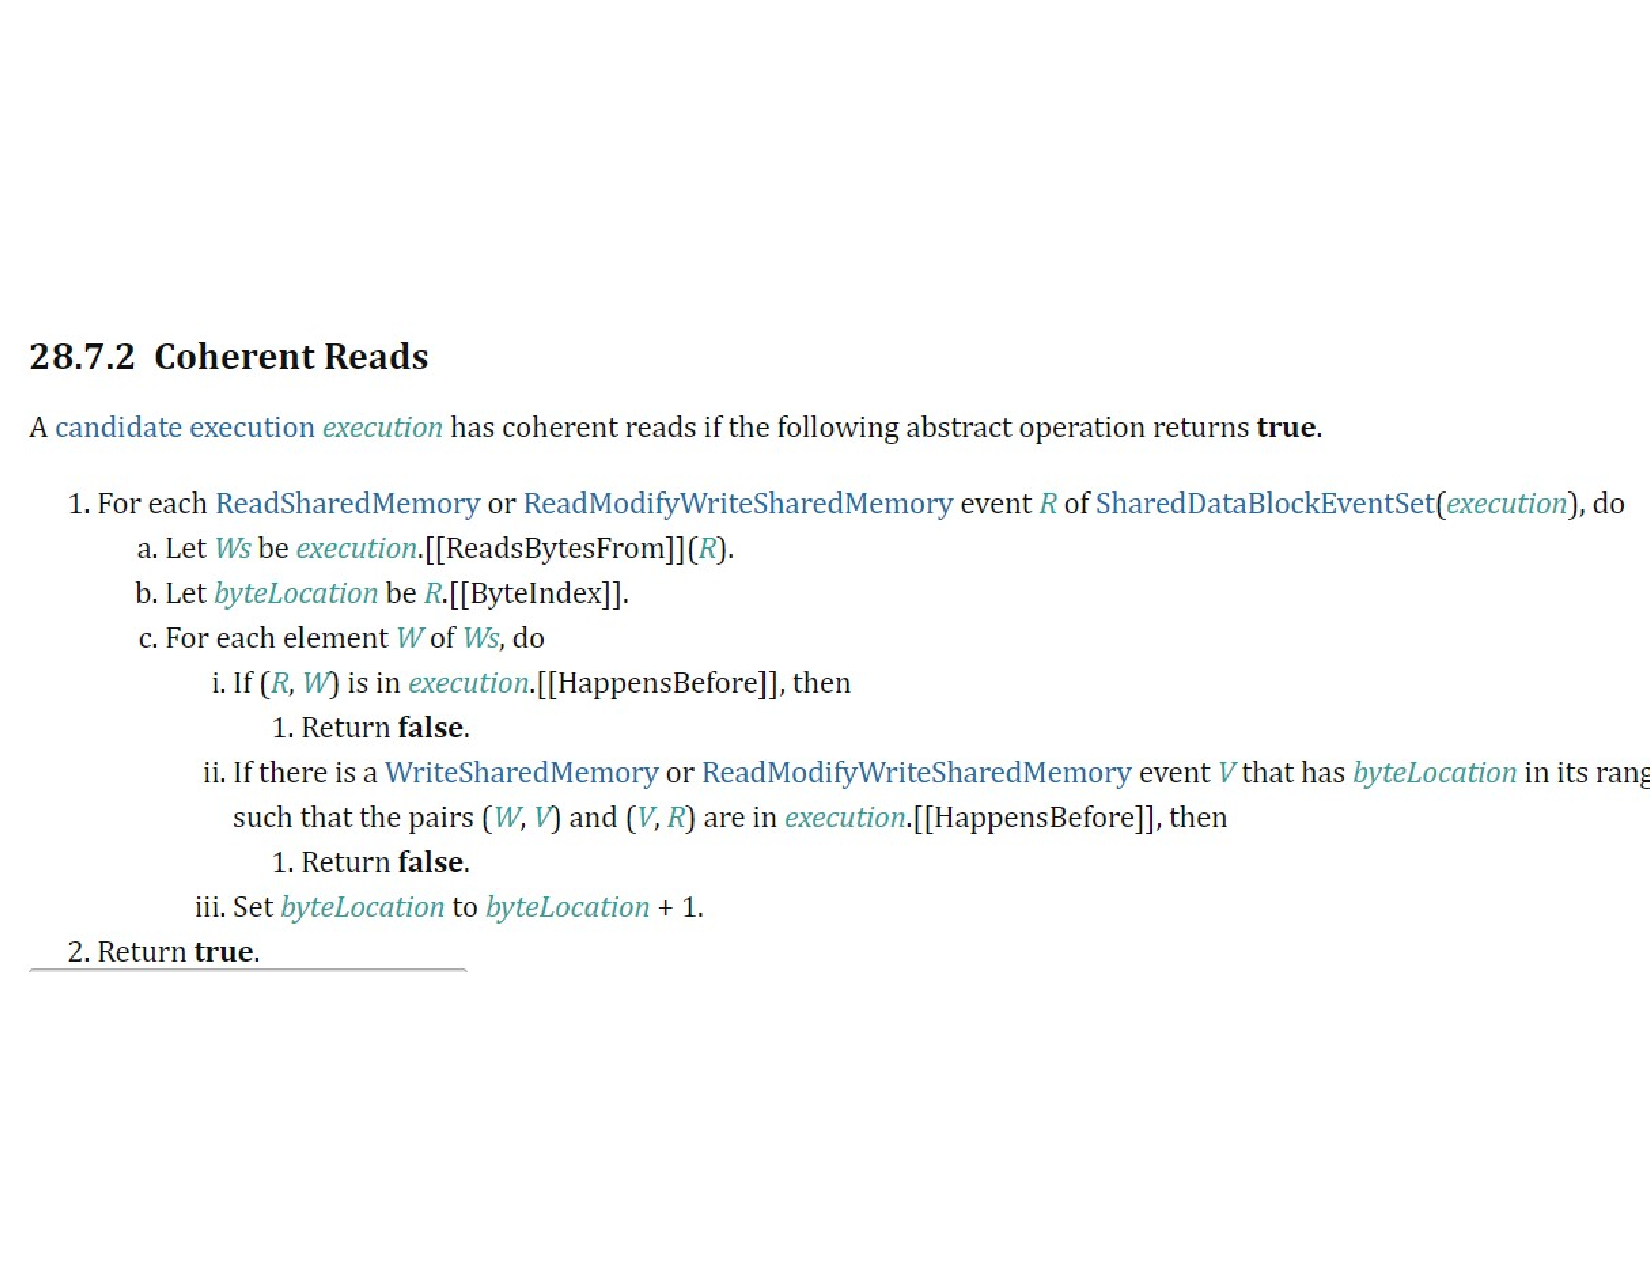
\includegraphics[scale=0.6]{4.ECMAScriptMemoryModel/ECMAScriptStdCoherentReads.pdf}
        \caption{The ECMAScript specification for Coherent Reads.}
        \label{model:Std1}
    \end{figure}
    Axiom in Figure~\ref{model:Std1} is specified as a return value to an abstract operation. While understanding this requires one to know the definitions for $Ws$, $execution$, $SharedDataBlockEventSet$ abstract operation, etc. we believe this is not needed as to understand what the axiom is about, which informally can be stated as below in two points:
    \begin{itemize}
        \item A read's value cannot come from a write that has happened after it. 
        \item A read's value cannot come from a write that has been overwritten by some other write.  
    \end{itemize}
    Axiomatically, we define the above two constraints using binary relations that we derive(also in some sense, take directly) from the specification. 
    
\paragraph{Certain Unnecessary Definitions}
    Certain abstract operations are not required to capture the semantics of the model. 
    One such example is in Figure~\ref{model:Std2}
    \begin{figure}[H]
        \centering 
        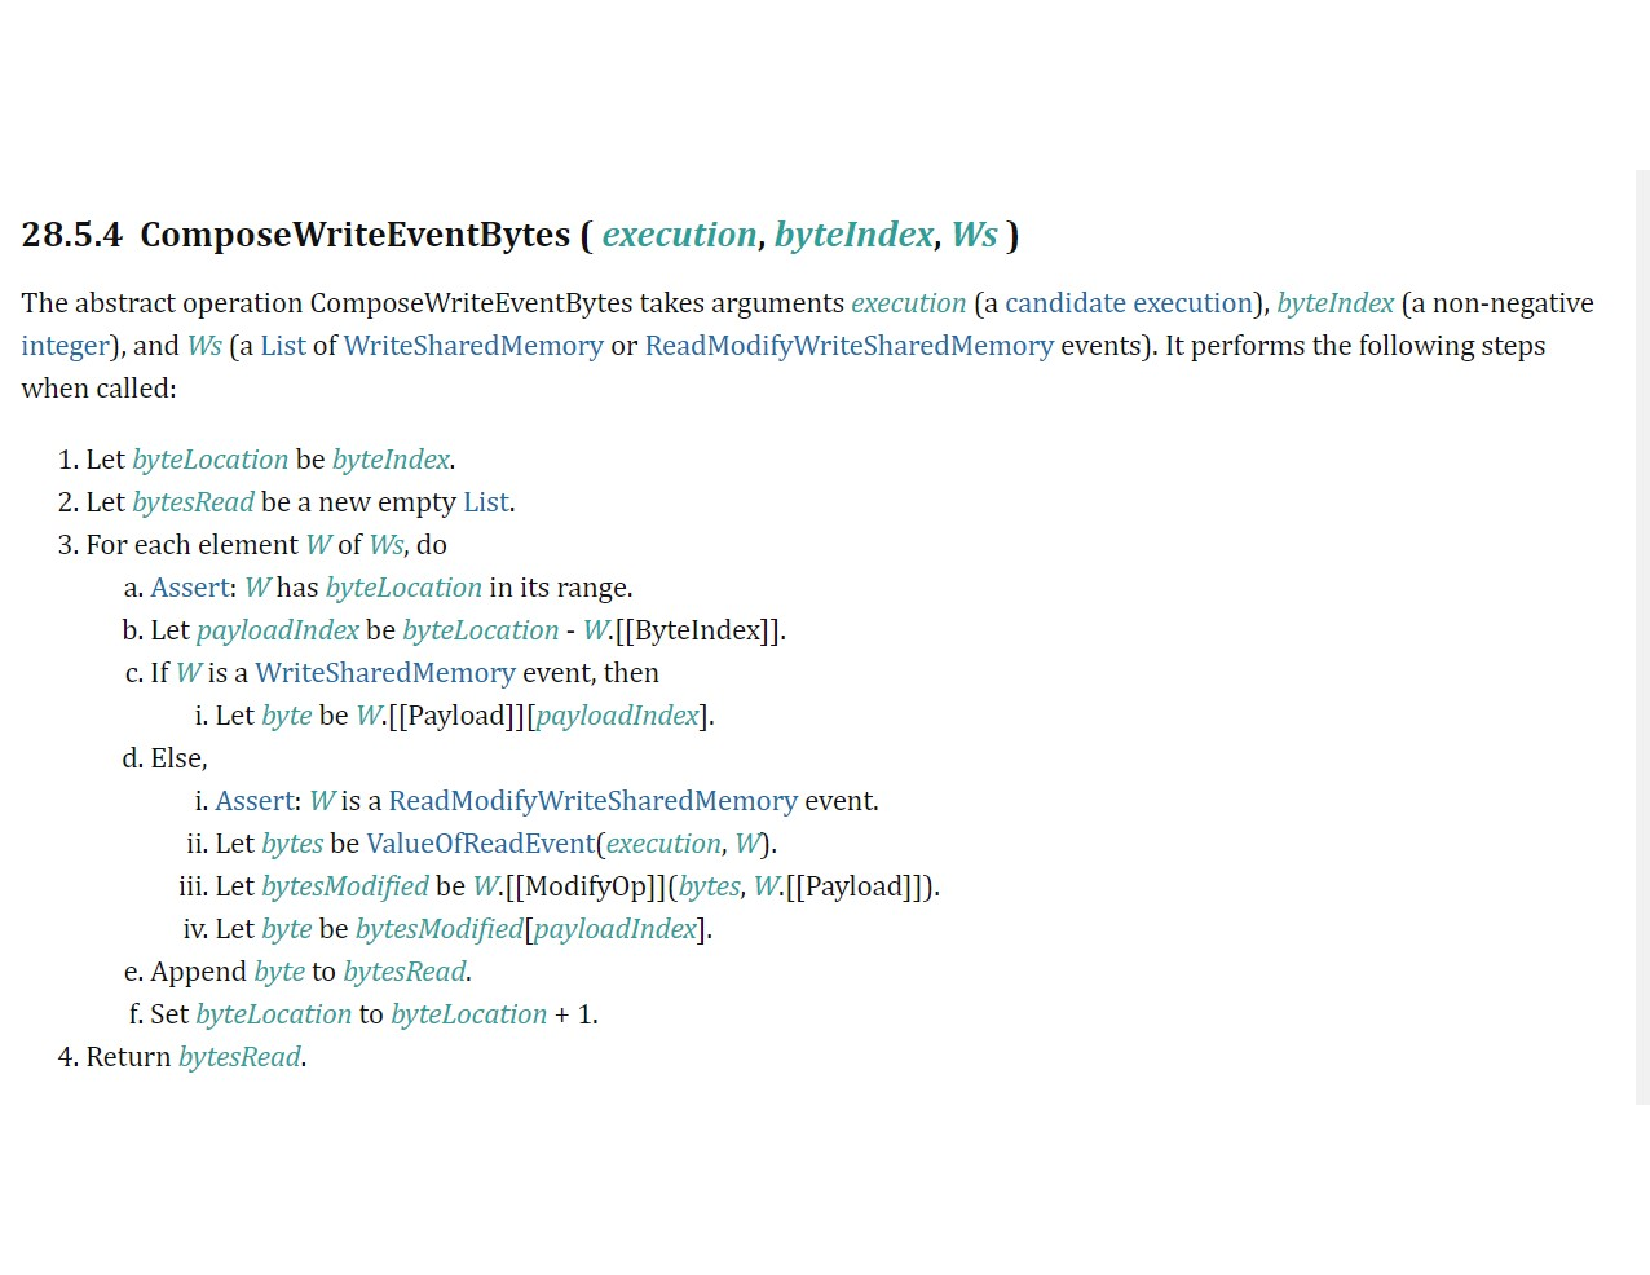
\includegraphics[scale=0.6]{4.ECMAScriptMemoryModel/ECMAScriptStd.pdf}
        \caption{The ECMAScript specification for Compose Write Event Bytes.}
        \label{model:Std2}
    \end{figure}
    Figure~\ref{model:Std2} is the definition of an abstract operation. To understand what this operation does, one must know the meaning of the terms $ModifyOp$, $Payload$, the list $Ws$, and also know what the argument $ByteIndex$ signifies. 
    In its essence, the above operation gives the read-values read by a single event by collecting the values from their corresponding writes. 
    We noticed that one need not know this operation nor understand its function as it does not play a role in the semantics of the model. 
    Other such abstract operations are $ValueOfReadEvent$ and $ValidChosenReads$. 

\paragraph{Still a bit verbose}
    
    The entire model, though algorithmic in its structure, is still quite verbose in its details, which makes it difficult to understand the model semantics. 
    Figure~\ref{model:Std3} is the std specification of another Axiom. 
    \begin{figure}[H]
        \centering 
        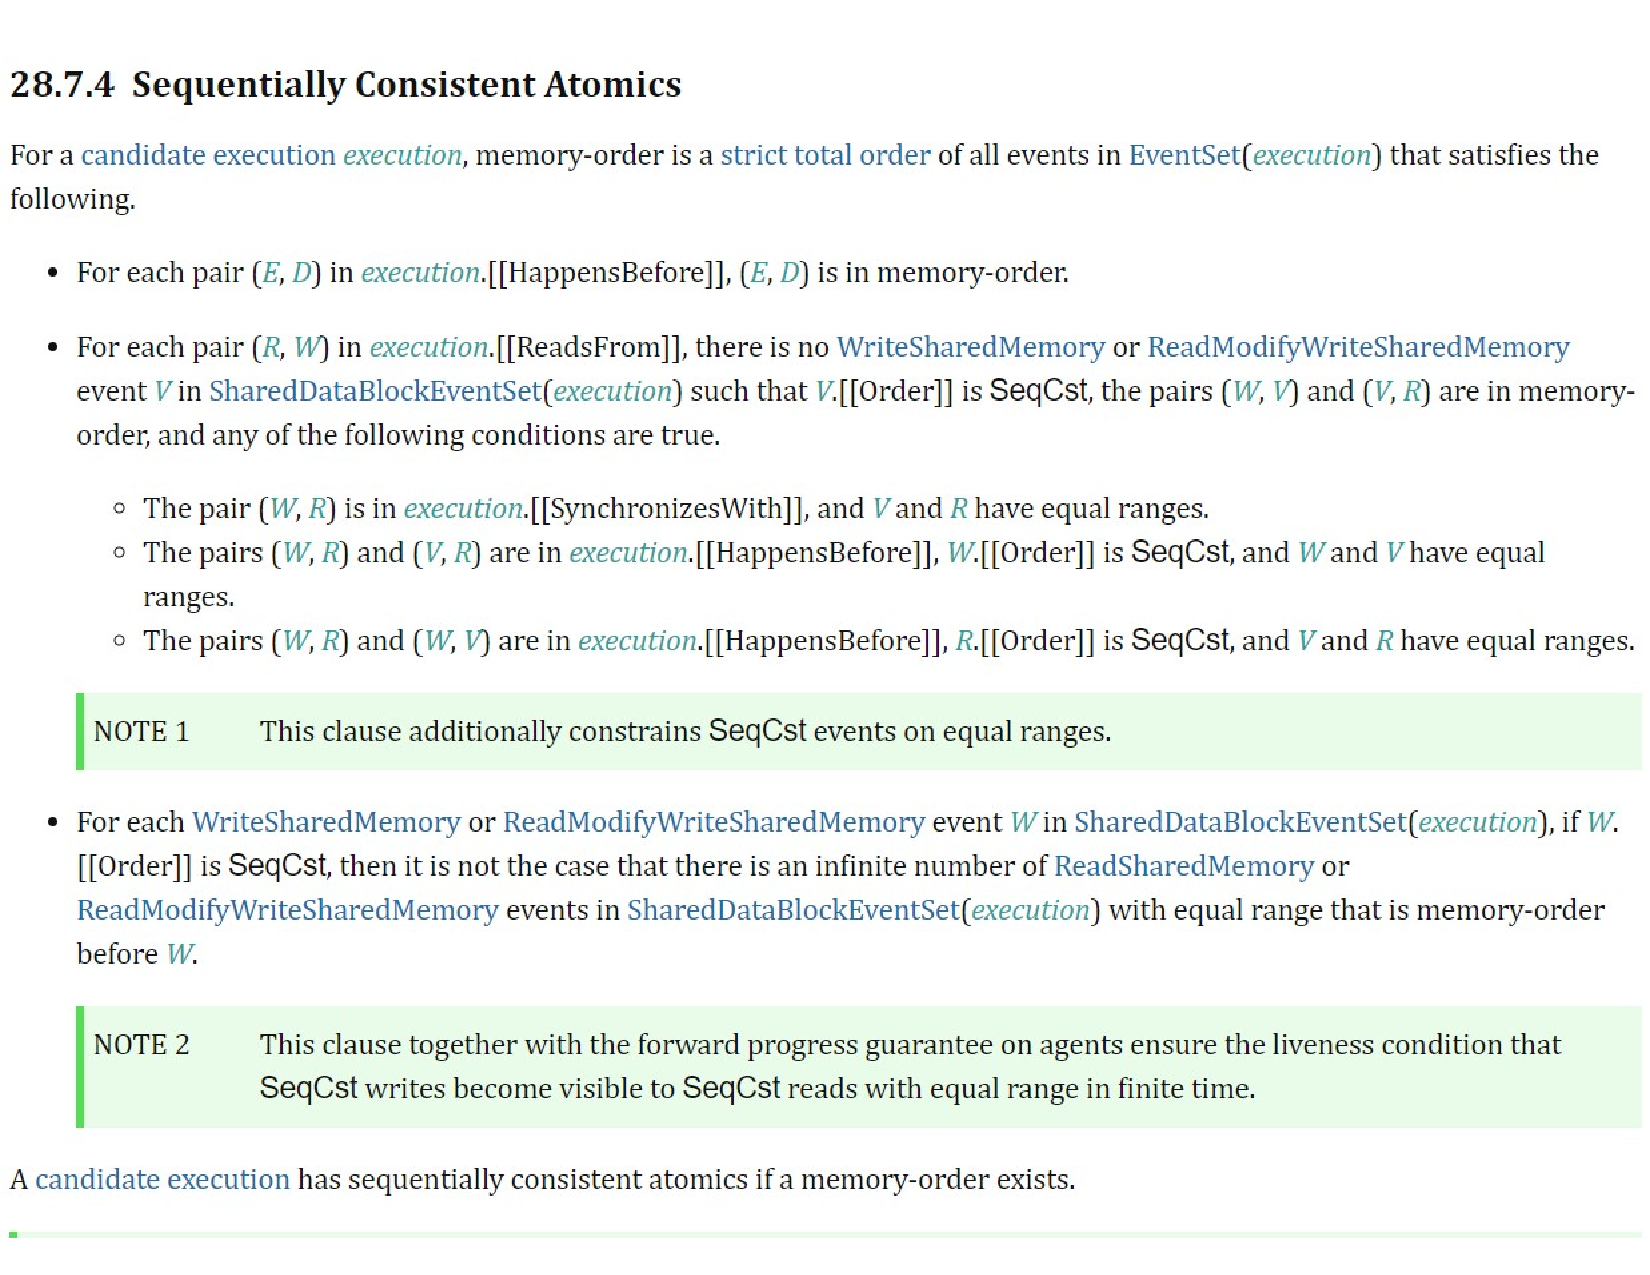
\includegraphics[scale=0.6]{4.ECMAScriptMemoryModel/ECMAScriptStdSeqCnsAt.pdf}
        \caption{The ECMAScript specification for Sequentially Consistent Atomics axiom.}
        \label{model:Std3}
    \end{figure}
    The axiom, though written concisely, in our view still makes it difficult to understand its purpose. 
    While the part after Note1 in Figure~\ref{model:Std3} is less of a semantic specification and more of a programming guideline while using 
    relaxed memory accesses.(one can make countless counter-examples for this.) 
    We reduced the above entire axiom into three main patterns using binary relations that should not exist in any execution of a program. 

Given the above concerns about the specification in the standard, we found the need to have a concise formal description of the model. 
In the following sections, we define what agents and events are, followed by several binary relations among different events.
